%%%%%%%%%%%%%%%%%%%%%%%%%%%%%%%%%%%%%%%%%%%%%%%%%%%%%%%%%%%%%%%%%%%%%%%%%%%%%%%%
%2345678901234567890123456789012345678901234567890123456789012345678901234567890
%        1         2         3         4         5         6         7         8

\documentclass[letterpaper, 10 pt, conference]{ieeeconf}  % Comment this line out if you need a4paper

%\documentclass[a4paper, 10pt, conference]{ieeeconf}      % Use this line for a4 paper

\IEEEoverridecommandlockouts                              % This command is only needed if 
                                                          % you want to use the \thanks command

\overrideIEEEmargins                                      % Needed to meet printer requirements.

% See the \addtolength command later in the file to balance the column lengths
% on the last page of the document

% The following packages can be found on http:\\www.ctan.org
\usepackage[pass]{geometry}
\usepackage{graphicx} % for pdf, bitmapped graphics files
\usepackage{subfigure}
%\usepackage{epsfig} % for postscript graphics files
\usepackage{mathptmx} % assumes new font selection scheme installed
\usepackage{times} % assumes new font selection scheme installed
\usepackage{amsmath} % assumes amsmath package installed
\usepackage{amssymb}  % assumes amsmath package installed

\graphicspath{{figures/}}
\setlength\fboxsep{0pt}
\setlength\fboxrule{0.2pt}
\newcommand{\norm}[1]{\lVert#1\rVert}
\newtheorem{proposition}{Proposition}
%\newtheorem{conjecture}{Conjecture}

\title{\LARGE \bf
Segregation of Multiple Heterogeneous Units in a Robotic Swarm
}


%TODO: completar (verificar no modelo original como os nomes devem ser colocados)
\author{Vinicius Graciano Santos \and Luciano C. A. Pimenta \and Luiz
  Chaimowicz% <-this % stops a space
  \thanks{This work was partially supported by CAPES, CNPq and Fapemig. We
    would like to thank Manish Kumar and Vijay Kumar for the
    discussions regarding swarm segregation.}%
  \thanks{V. G. Santos and L. Chaimowicz are with the Vision and
    Robotics Laboratory (VeRLab), Computer Science Department,
    Universidade Federal de Minas Gerais, Brazil. {\tt\small emails:
      \{vgs, chaimo\}@dcc.ufmg.br}} \thanks{L. C. A. Pimenta is with
    the Department of Electronic Engineering, Universidade Federal de
    Minas Gerais, Brazil. {\tt\small email: lucpim@cpdee.ufmg.br}}%
}


\begin{document}



\maketitle
\thispagestyle{empty}
\pagestyle{empty}


%%%%%%%%%%%%%%%%%%%%%%%%%%%%%%%%%%%%%%%%%%%%%%%%%%%%%%%%%%%%%%%%%%%%%%%%%%%%%%%%
\begin{abstract}
  Several natural systems adopt self-sorting mechanisms based on
  segregative behaviors. Among these, cell segregation is of
  particular interest since it plays an important role in the
  formation of tissues, organs, and living organisms. The Differential
  Adhesion Hypothesis states that cells naturally segregate because of
  differences in affinity, which lead similar cells to strongly adhere
  to each other. By exploring this principle, we propose a controller
  that can segregate a heterogeneous swarm of robots according to the
  characteristics of each agent, such that similar robots form
  homogeneous teams and dissimilar robots are segregated. We apply
  LaSalle's Invariance Principle to show convergence and perform
  simulated experiments in order to demonstrate the robustness and
  effectiveness of the proposed controller. Results show that our
  approach allows a swarm of multiple heterogeneous robots to
  segregate in a coherent and smooth fashion, without any inter-agent
  collisions.
\end{abstract}

%%%%%%%%%%%%%%%%%%%%%%%%%%%%%%%%%%%%%%%%%%%%%%%%%%%%%%%%%%%%%%%%%%%%%%%%%%%%%%%%
\section{INTRODUCTION}
Swarm robotics studies multi-agent systems which consist of a large
number of relatively simple robots. These agents can solve complex
problems by relying on system-level properties such as robustness,
flexibility, and scalability~\cite{Sahin:04}. Most researchers in
swarm robotics usually focus on homogeneous systems, in which all
robots have the same characteristics. However, several applications of
multi-robot and swarm systems require the use of heterogeneous teams
of agents in order to fulfill a given mission, as sometimes it is not
possible to integrate all of the required sensing and actuation
capabilities for the task in a single robot. These heterogeneous
systems are specially useful on cooperative assignments such as search
and rescue, surveillance, perimeter protection, and transportation of
large objects.

In some cases, heterogeneous agents must be able to organize
themselves in a specific manner to carry out their assigned tasks. For
instance, robots that gather distinct types of materials may need to
form teams which can maximize the gathering of a particular
resource. One strategy would be to sort agents according to their
specialization, such that gatherers of similar materials stay in the
same team. Afterwards, these groups can be deployed to different
regions where a specific resource is abundant. We can say that such
system shows a segregative behavior since the sorting process leads
dissimilar agents into distinct teams.

Segregation is a particular sorting mechanism that is common in
nature, being widely used by many individuals such as cells and
animals to shape these populations into tissues as well as societies,
respectively. This behavior has been extensively studied by
biologists, but few robotics researchers have tried to simulate it on
large swarm systems. Therefore, we propose in this paper a controller
that can segregate a heterogeneous robotic swarm according to the
characteristics of each robot, such that similar robots form a
cohesive team, and dissimilar ones are separated from each other. We
base our approach on the differential potential
concept~\cite{Kumar:10}, an analogy for multi-agent systems of the
biological mechanisms by which cells segregate, extending it to
multiple groups. Furthermore, we employ LaSalle's Invariance Principle
to demonstrate convergence and present several simulated experiments
in 2D and 3D spaces, which validate the proposed controller.

This paper is organized as follows: Section~\ref{sec:related_work}
discusses related work on swarm control and segregation. In
Section~\ref{sec:methodology}, we present our controller which is able
to achieve segregation in swarm systems. Experimental results in
simulated scenarios are detailed in Section~\ref{sec:experiments}, and
Section~\ref{sec:conclusion} closes the paper with our conclusions and
directions for future work.
%%%%%%%%%%%%%%%%%%%%%%%%%%%%%%%%%%%%%%%%%%%%%%%%%%%%%%%%%%%%%%%%%%%%%%%%%%%%%%%%
\section{RELATED WORK}
\label{sec:related_work}

Reynolds~\cite{Reynolds:87} was one of the first researchers to
realistically simulate the movement of a swarm of agents, more
specifically a flock of birds, known as \textit{boids}. His algorithm
relies on three simple steering rules that an agent applies based on
the information of its surrounding neighbors: \textit{separation},
which avoids collisions; \textit{alignment}, which steers the agents
towards their average heading; and \textit{cohesion}, which moves the
agents towards their average position. Such interactions can be
modeled as a special case of the social potential field method
\cite{Reif:99}, an extension of the classical artificial potential
field technique~\cite{Khatib:85} that specifically deals with
multi-agent systems. These works have been widely employed as
foundations to several methodologies on the control of robotic swarms,
such as behavior-based~\cite{Balch:98},
leader-follower~\cite{Leonard:01,Tanner:04}, hierarchical abstractions
\cite{Belta:04,Santos:11a}, hydrodynamic-based~\cite{Pimenta:13}, and
others~\cite{Olfati-Saber:06,Tanner:07}.

Segregation is a natural phenomenon that appears in several
biological systems. For instance, ants sort their brood in annular
patterns in which distinct broods tend to be placed at particular
annuli~\cite{Franks:92}. Another example is cellular segregation,
which is of central importance in embryogenesis, as the formation of
many tissues require an initial subdivision of cells into regions,
each with specific characteristics that will allow particular cell
types to be generated~\cite{Eduard:12}. Steinberg's
\textit{Differential Adhesion Hypothesis}~\cite{Steinberg:63} states
that differences in cell adhesion generate mechanical forces which
drive cellular segregation. In other words, a cell population
experience stronger cohesive forces from similar cells than from
dissimilar ones, and this imbalance is responsible for the segregative
behavior~\cite{Eduard:12}.

Robotics researchers have mostly focused on segregation as a mechanism
by which robots sort a collection of objects (e.g.,
see~\cite{Deneubourg:91}), but some authors have specifically dealt
with segregation of heterogeneous agents. For example,
Gro\ss~\cite{Gross:09} discussed a motor schema that allowed mobile
robots to self-organize into annular structures. A distributed
controller considers robots as having distinct virtual sizes, and
local interactions make ``larger'' robots move outwards. This
procedure was inspired by the \textit{Brazil Nut Effect}, a granular
convection phenomenon by which a mixture of granular material
subjected to vibrations will lead its largest particles to the
surface. This work was later extended to consider real e-puck
robots~\cite{Chen:12}. In spite of the interesting results, the
controller requires all robots to share a common target in order to
simulate the gravitational forces responsible for the granular
convection. This implies that a centralized broadcast or a consensus
algorithm must be executed previously. Based on Steinberg's
work~\cite{Steinberg:63}, Kumar et al.~\cite{Kumar:10} proposed the
\textit{differential potential concept}, which asserted that agents
should experience different magnitudes of potential while interacting
with agents of distinct types in order to achieve
segregation. Stability analysis as well as convergence proofs were
presented. Nevertheless, their approach is limited to only two types
of robots, and the use of multiple types easily leads the system to
local minima where segregation does not occur, a result which we have
seen in many experiments performed with their controller. Finally, in
a previous work~\cite{Santos:12}, we maintained segregation among
multiple robot groups during navigation by using velocity
obstacles~\cite{Fiorini:98}, but our method depends on teams being
already segregated at the initial time step.

In the present work, we are interested in developing proper mechanisms
that ensure segregation in the case of multiple robot types. We tackle
this problem by adapting and extending Kumar's work~\cite{Kumar:10} to
deal with this scenario. Besides, we also introduce a new metric in
order to define segregation in a more convenient way, which can be
easily verified. Apart from 2D simulations, we explore our
controller's behavior in 3D spaces as well.

%%%%%%%%%%%%%%%%%%%%%%%%%%%%%%%%%%%%%%%%%%%%%%%%%%%%%%%%%%%%%%%%%%%%%%%%%%%%%%%%
\section{METHODOLOGY}
\label{sec:methodology}

We consider a set of fully actuated mobile agents whose dynamics are
given by the double integrator
\begin{equation}
  \label{eq:dynamics}
  \dot{q}_i = v_i \;\;\text{and}\;\; \dot{v}_i = u_i \hspace{2em} i \in \Upsilon = \{1,2,\dots,n\},
\end{equation}
in which $q_i \in \mathbb{R}^p$, $v_i \in \mathbb{R}^p$, and $u_i \in
\mathbb{R}^p$ denote the position, velocity, and control input of
robot $i$, respectively. This set of mobile agents consists of
different types of robots, which we represent by the partition $\tau =
\{\tau_1,\tau_2,\dots,\tau_m \}$, where each $\tau_k \subset \Upsilon$
contains all agents of type $k$. We assume that $\forall j,k: \, j
\neq k \to \tau_j \cap \tau_k = \emptyset$ and $\forall
j,k:|\tau_j|=|\tau_k|$, i.e., each robot is uniquely assigned to a
single type and the type partition is fully balanced, respectively.

Our objective is to synthesize a controller that can sort robots of different
types into $m$ distinct clusters in the workspace, such that each
cluster contains agents of a single type only. We refer to the latter
as the \textit{segregation problem}, and a control system which solves
this problem is said to display a \textit{segregative behavior}.

\subsection{Control Law}

Given a population of $n$ heterogeneous mobile robots with partition
$\tau$ and dynamics specified by (\ref{eq:dynamics}), we propose the
following control law:
\begin{equation}
  \label{eq:controller}
  u_i = - \sum_{j \neq i} \nabla_{q_i} U_{ij}(\norm{q_i - q_j}) - \sum_{j \neq i} (v_i - v_j),
\end{equation}
in which $U_{ij}(\norm{q_i-q_j})$ is an artificial potential function
that rules the interaction between agents $i$ and $j$,
$\norm{q_i-q_j}$ is the Euclidean norm of the vector $q_i-q_j$, and
$\nabla_{q_i}$ is the gradient with respect to the coordinates of
agent $i$. The first term represents the resultant force that acts on
robot $i$ given its interactions with all other agents, whereas the
second term serves as damping and causes robots to match their
velocities. This kind of controller equation is a common approach for
potential-based swarm
systems~\cite{Kumar:10,Leonard:01,Olfati-Saber:06}.

The artificial potential field $U_{ij}:\mathbb{R} \to \mathbb{R}_{>0}$
is a function of the relative distance between a pair of agents that
we express as
\begin{equation}
  \label{eq:potential}
  U_{ij}(\norm{q_{ij}}) = \alpha\left(\frac{1}{2} (\norm{q_{ij}} - d_{ij})^2 + \ln{\norm{q_{ij}}} + \frac{d_{ij}}{\norm{q_{ij}}}\right),
\end{equation}
in which $\alpha$ is a scalar control gain, $q_{ij}$ is a shortened
form of writing $q_i-q_j$ (i.e., $q_{ij}=q_i-q_j$), and $d_{ij}$ is a
positive parameter that will be described later. The initial
conditions and dynamics of the system exclude the situations where
$\norm{q_{ij}} = 0$, in which ($\ref{eq:potential}$) is
undefined. Furthermore, as we will show later, if robots do not
collide at the initial configuration then there will be no collisions
through all time steps.

Although there are $m$ distinct types of robots involved in the
system, each agent classifies its neighbors as being either of its own
type or of a different type. This means that agents see the system
through a binary filter which reduces possible robot interactions to
only two kinds thereof: among robots of the same type and among robots
of distinct types. Formally, we say that an agent $i$ has a local type
partition
\begin{equation}
  \label{eq:local_types}
  ^i\tau = \{\tau_k, \Upsilon \setminus \tau_k\} \hspace{1em} i \in \tau_k,
\end{equation}
where $\tau_k \in \tau$, and $\Upsilon \setminus \tau_k$ represents the set difference.

\begin{figure}[thpb]
  \centering
  \subfigure[Inter-agent potential.]{
    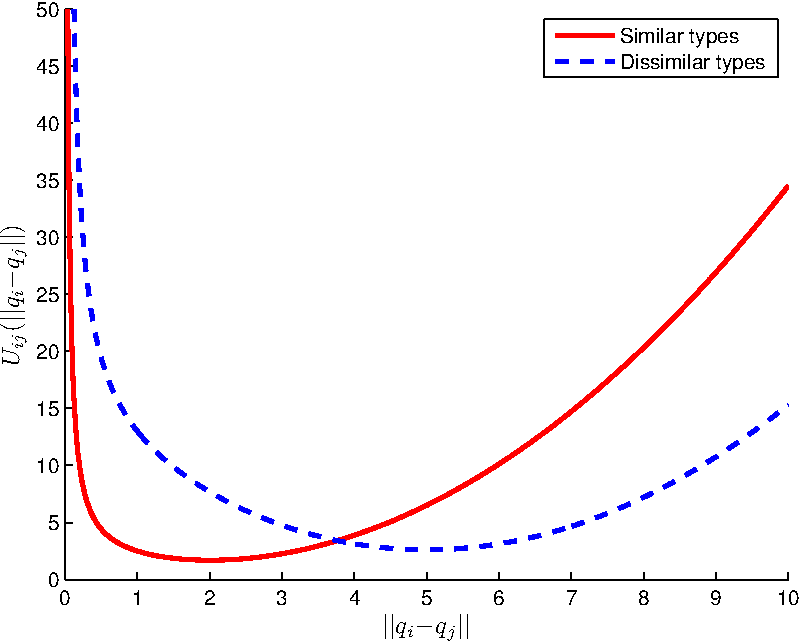
\includegraphics[width=\columnwidth]{potential.pdf}
    \label{fig:potential}} 
  \subfigure[Inter-agent force.]{
    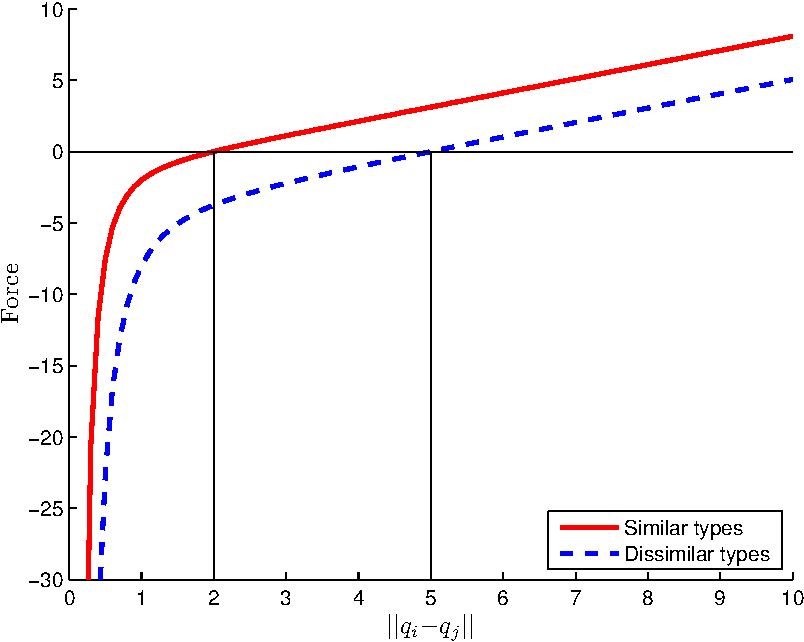
\includegraphics[width=\columnwidth]{force.pdf}
    \label{fig:force}}
  \caption{Plot of the artificial potential field $U_{ij}(\norm{q_j -
      q_i})$ and its underlying forces given $d_{AA}=2$ and $d_{AB}=5$.}
  \label{fig:plots}
\end{figure}

In order to segregate robots, we apply the \textit{differential
  potential} concept, i.e., pairs of dissimilar agents experience
different magnitudes of potential than pairs of similar
agents~\cite{Kumar:10}. We can accomplish this by defining the
parameter $d_{ij}$ of (\ref{eq:potential}) according to the local type
partition $^i\tau$.
\begin{equation}
  \label{eq:dij}
  d_{ij}(^i\tau) =
  \begin{cases}
    d_{AA},& \text{if } i \in \tau_k \text{ and } j \in \tau_k \\
    d_{AB},& \text{if } i \in \tau_k \text{ and } j \not\in \tau_k
  \end{cases}
\end{equation}

Equation (\ref{eq:dij}) states that interactions among similar and
dissimilar types of robots are ruled by $d_{AA}$ and $d_{AB}$,
respectively. Thus, the system exhibits a segregative behavior when we
choose values for these parameters such that
\begin{equation}
  \label{eq:restriction}
  0 < d_{AA} < d_{AB}.
\end{equation}

We show in Figure \ref{fig:potential} a plot of the artificial
potential function $U_{ij}(\norm{q_{ij}})$, whose minimum is located
at $\norm{q_{ij}} = d_{ij}$. Furthermore, we depict the interaction
forces among a pair of robots in Figure \ref{fig:force}, in which
constraint (\ref{eq:restriction}) holds true. The latter plot actually
represents the scalar part of the gradient
% TODO: verificar sinais
\begin{equation}
  \label{eq:gradient}
  \nabla U_{ij}(\norm{q_{ij}}) = \alpha \left(\norm{q_{ij}} - d_{ij} + \frac{1}{\norm{q_{ij}}} - \frac{d_{ij}}{\norm{q_{ij}}^2}\right) \frac{q_{ij}}{\norm{q_{ij}}},
\end{equation}
in which we ignore the normalized vector term. It is easy to see that,
at any given distance, forces among agents of similar types are
greater than those among different types. Therefore, our controller
respects the differential potential concept~\cite{Kumar:10}, and
effectively implements an approximation of Steinberg's differential
adhesion model~\cite{Steinberg:63}.

\subsection{Controller Analysis}
In this section, we analyze the convergence of the multi-agent system
when using the proposed control law. We start with the definition of
the Lyapunov function
\begin{equation}
  \label{eq:lyapunov}
  V(\mathbf{q},\mathbf{v}) = U(\mathbf{q}) + \frac{1}{2} \mathbf{v}^\intercal\mathbf{v},
\end{equation}
where $\mathbf{q} \in \mathbb{R}^{np}$ and $\mathbf{v} \in
\mathbb{R}^{np}$ are stacked vectors whose components are the
configurations and velocities of all robots, respectively, and
$U(\mathbf{q}): \mathbb{R}^{np} \to \mathbb{R}_{>0}$ is the collective
artificial potential function, which we write as
\begin{align}
  \label{eq:collective_potential}
  U(\mathbf{q}) &= \frac{1}{2} \sum_{\tau_k \in \tau} \sum_{i \in
    \tau_k} \sum_{j \in \tau_k, j \neq i} U_{ij}(\norm{q_i - q_j})
  \nonumber\\
  &+ \frac{1}{2} \sum_{\tau_k \in \tau} \sum_{i \in \tau_k} \sum_{j
    \in \Upsilon \setminus \tau_k} U_{ij}(\norm{q_i - q_j}).
\end{align}
Thus, we can model the collective dynamics of the system:
\begin{align}
  \label{eq:collective_dynamics_a}
  \dot{\mathbf{q}} &= \mathbf{v} \\
  \label{eq:collective_dynamics_b}
  \dot{\mathbf{v}} &= -\nabla U(\mathbf{q}) - \hat{L}(\mathbf{q})\mathbf{v},
\end{align}
in which $\hat{L}(\mathbf{q}) = L(\mathbf{q}) \otimes I_p $ is the
Kronecker product of the system's graph Laplacian $L(\mathbf{q})$ and
the $p \times p$ identity matrix $I_p$ (for a complete description,
see~\cite{Olfati-Saber:06}). These definitions let us introduce the
proposition below.

\begin{proposition}
  Assuming that the underlying adjacency graph of the system is
  complete at all times, for any initial condition that belongs to the
  level set $\Omega_C = \{(\mathbf{q},\mathbf{v}) \mid
  V(\mathbf{q},\mathbf{v}) \leq C\}$, with $C > 0$, a heterogeneous
  system with type partition $\tau$ on $n$ mobile agents, whose
  dynamics and control laws are respectively given by
  (\ref{eq:dynamics}) and (\ref{eq:controller}), asymptotically
  converges to the largest invariant set in $\Omega_I =
  \{(\mathbf{q},\mathbf{v}) \in \Omega_C \mid \dot{V}(\mathbf{q}) =
  0\}$, without any inter-agent collisions. At the largest invariant
  set in $\Omega_I$, the velocity of each agent is bounded, all
  velocities match, and the system's collective potential reaches a
  local minimum.
\end{proposition}

\begin{proof}
  We aim to demonstrate that $\dot{V}(\mathbf{q},\mathbf{v}) \leq 0$
  in order to apply LaSalle's Invariance Principle to show
  convergence. To achieve this, we can differentiate $V(\mathbf{q},
  \mathbf{v})$ with respect to time and then substitute
  (\ref{eq:collective_dynamics_a}) and
  (\ref{eq:collective_dynamics_b}) as follows:
  \begin{align}
    \label{eq:proof}
    \dot{V}(\mathbf{q},\mathbf{v}) &= \dot{\mathbf{q}}^\intercal
    \nabla
    U(\mathbf{q}) + \mathbf{v}^\intercal \dot{\mathbf{v}} \nonumber\\
    & = \mathbf{v}^\intercal \nabla
    U(\mathbf{q}) + \mathbf{v}^\intercal (-\nabla U(\mathbf{q}) - \hat{L}(\mathbf{q})\mathbf{v}) \nonumber\\
    & = - \mathbf{v}^\intercal \hat{L}(\mathbf{q})\mathbf{v} =
    -\frac{1}{2}\sum_i\sum_j\norm{v_j - v_i}^2 \leq 0.
  \end{align}
  The last step holds because the system's adjacency graph is
  complete~\cite{Olfati-Saber:06}. From LaSalle's Invariance
  Principle, all initial conditions that lie on $\Omega_C$ will lead
  the system to the largest invariant set in $\Omega_I$, where
  $\dot{V}(\mathbf{q},\mathbf{v}) = 0$. Therefore, (\ref{eq:proof})
  implies that all velocities match, i.e., $\forall i,j: v_i =
  v_j$. By (\ref{eq:lyapunov}) and (\ref{eq:collective_dynamics_a}),
  we have $\mathbf{v}^\intercal \mathbf{v} \leq 2C$ because
  $V(\mathbf{q}, \mathbf{v}) \leq C$, which leads to
  $\norm{\mathbf{v}} \leq \sqrt{2C}$. Consequently, all velocities are
  bounded by $\sqrt{2C}$ as well. Matching velocities imply that
  inter-agent distances remain constant, hence $\forall i,j:
  \dot{q}_{ij} = \mathbf{0}$, and thus
  \begin{align}
    \label{eq:collective_grad_time}
    \dot{U}(\mathbf{q}) &= \frac{1}{2} \sum_{\tau_k \in \tau} \sum_{i
      \in \tau_k} \sum_{j \in \tau_k, j \neq i} \dot{q}_{ij}^\intercal
    \nabla_{q_{ij}} U_{ij}(\norm{q_{ij}})
    \nonumber\\
    &+ \frac{1}{2} \sum_{\tau_k \in \tau} \sum_{i \in \tau_k} \sum_{j
      \in \Upsilon \setminus \tau_k} \dot{q}_{ij}^\intercal \nabla_{q_{ij}}
    U_{ij}(\norm{q_{ij}}) = 0,
  \end{align}
  which implies that $U(\mathbf{q})$ is constant at the steady
  state. Moreover, as $\hat{L}(\mathbf{q})\mathbf{v} = \mathbf{0}$
  because of matching velocities, we can reduce
  (\ref{eq:collective_dynamics_b}) to
  \begin{equation}
    \label{eq:stable_state_dyn}
    \dot{\mathbf{v}} = -\nabla U(\mathbf{q}).
  \end{equation}
  Therefore, $\nabla U(\mathbf{q})$ must be the zero vector, as
  otherwise the collective potential would reach a lower value
  instead of being constant. This implies that the system has reached
  a local minimum and velocities must not change.

  Finally, assume that robots $i$ and $j$ collide, i.e.,
  $\norm{q_{ij}} = 0$. We can see from (\ref{eq:potential}) and
  (\ref{eq:collective_potential}) that this would take $U(\mathbf{q})
  \to \infty$, but this contradicts the fact that $V(\mathbf{q}, \mathbf{v})
  \leq C$. Hence, no agent collides with each other.
\end{proof}
\subsection{Metric}
In order to measure segregation among clusters quantitatively, we
propose a metric that is based on the pairwise intersection area of
their convex hulls:
\begin{equation}
  \label{eq:metric}
  M(\mathbf{q}, \tau) = \sum_{\tau_k \in \tau} \sum_{\tau_l \in \tau, l \neq k} A\left(CH(\bigcup_{i \in \tau_k}q_i) \bigcap CH(\bigcup_{j \in \tau_l} q_j) \right),
\end{equation}
in which $A(Q)$ and $CH(Q)$ denote the area and the convex hull of set
$Q$, respectively. We have chosen this metric because the convex hull
can be used as a simple and well-defined shape representation of a
cluster. This means that segregation occurs when there is no overlap
among clusters. In other words, we say that the system is fully
segregated when $M(\mathbf{q}, \tau)$ approaches zero.

%%%%%%%%%%%%%%%%%%%%%%%%%%%%%%%%%%%%%%%%%%%%%%%%%%%%%%%%%%%%%%%%%%%%%%%%%%%%%%%%
\section{EXPERIMENTS}
\label{sec:experiments}

We executed a sequence of simulations in order to study the
performance and feasibility of our proposed approach. We first present
their results according to metric $M(\mathbf{q}, \tau)$ and then
display some snapshots of these experiments. Finally, we close the
section with a discussion on the behavior of the system as well as on
particular details of our method.

\subsection{Simulations}

\begin{figure}[htpb]
  \centering
  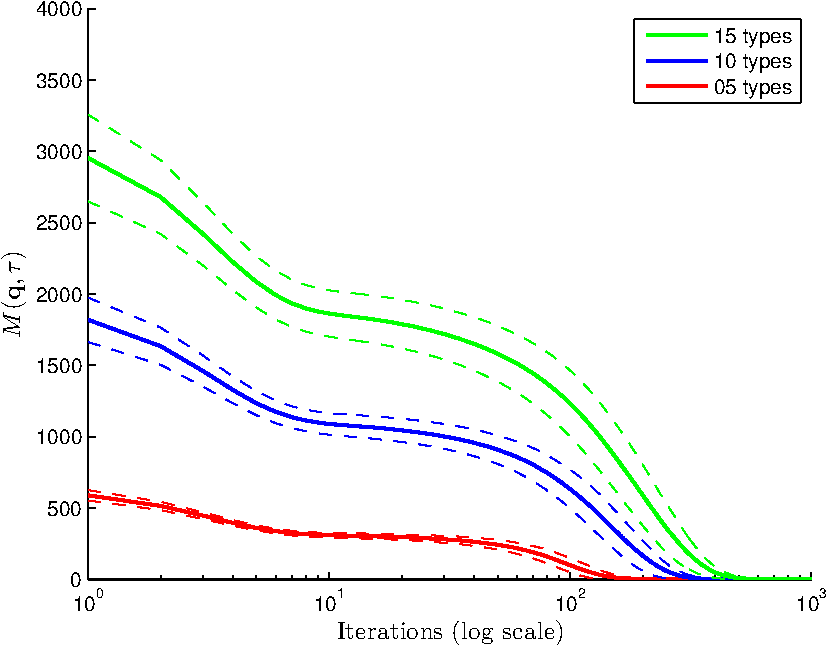
\includegraphics[width=\columnwidth]{chull.pdf}
  \caption{Mean intersection area of convex hulls for $100$
    experiments with a varying number of robot types. Dashed lines
    represent one standard deviation from the mean.}
  \label{fig:chull}
\end{figure}

We have performed an extensive series of simulations in order to
analyze our controller under metric $M(\mathbf{q}, \tau)$. Each
simulation consisted of $150$ robots and a varying number of agent
types. At the initial state, all velocities were set to zero, and
robots were positioned according to a two-dimensional uniform
distribution, which is independent of a robot's type. Additionally, we
have set $d_{AA} = 2$ and $d_{AB} = 5$ for all experiments. We present
in Figure \ref{fig:chull} the mean and standard deviation of
$M(\mathbf{q},\tau)$ among $100$ experiments given these initial
conditions. In all cases, both the mean and standard deviation
approach zero as the number of iterations increase. Moreover, systems
with less types tend to achieve segregation faster than those with
more types. This is expected, as given a fixed number of robots, the
use of a large number of types would result in few robots per
cluster, which in turn would lower the magnitude of the resultant
force towards it.

\begin{figure*}[thpb]
\centering
\subfigure[5 heterogeneous types.]{
  \fbox{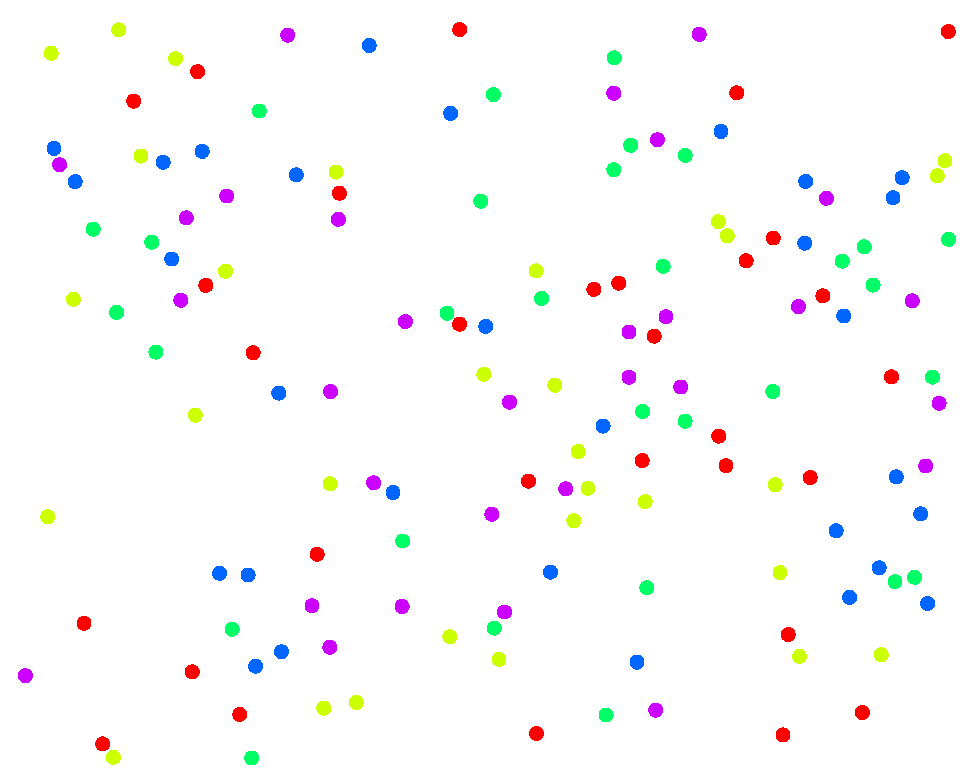
\includegraphics[width=0.15\paperwidth]{05types-1.pdf}}
  \fbox{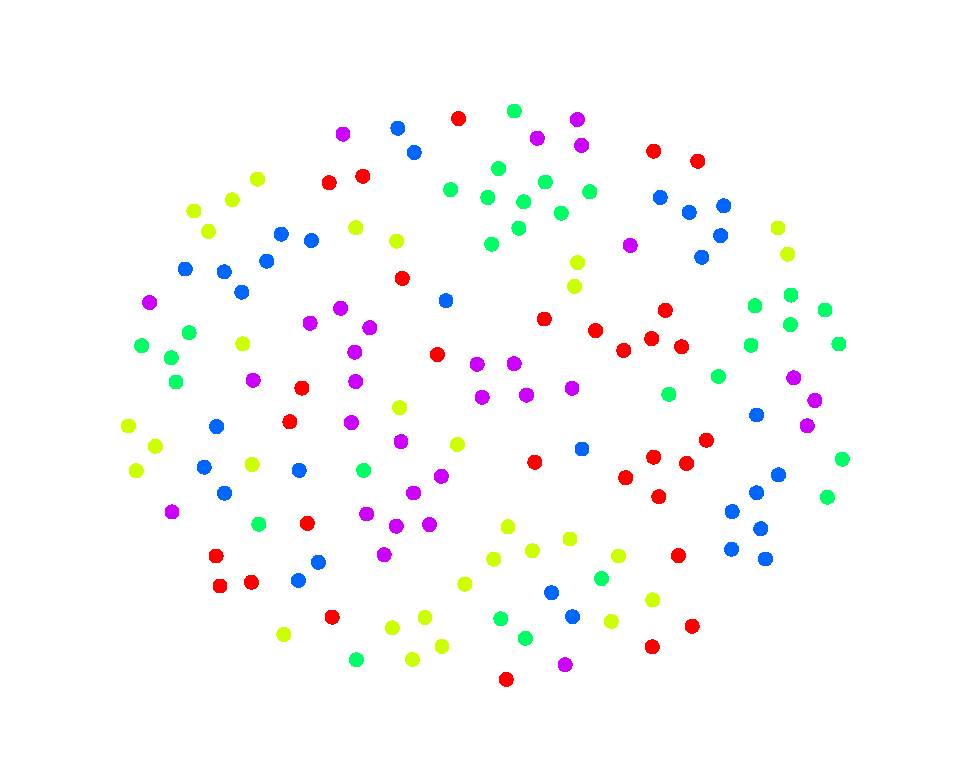
\includegraphics[width=0.15\paperwidth]{05types-2.pdf}}
  \fbox{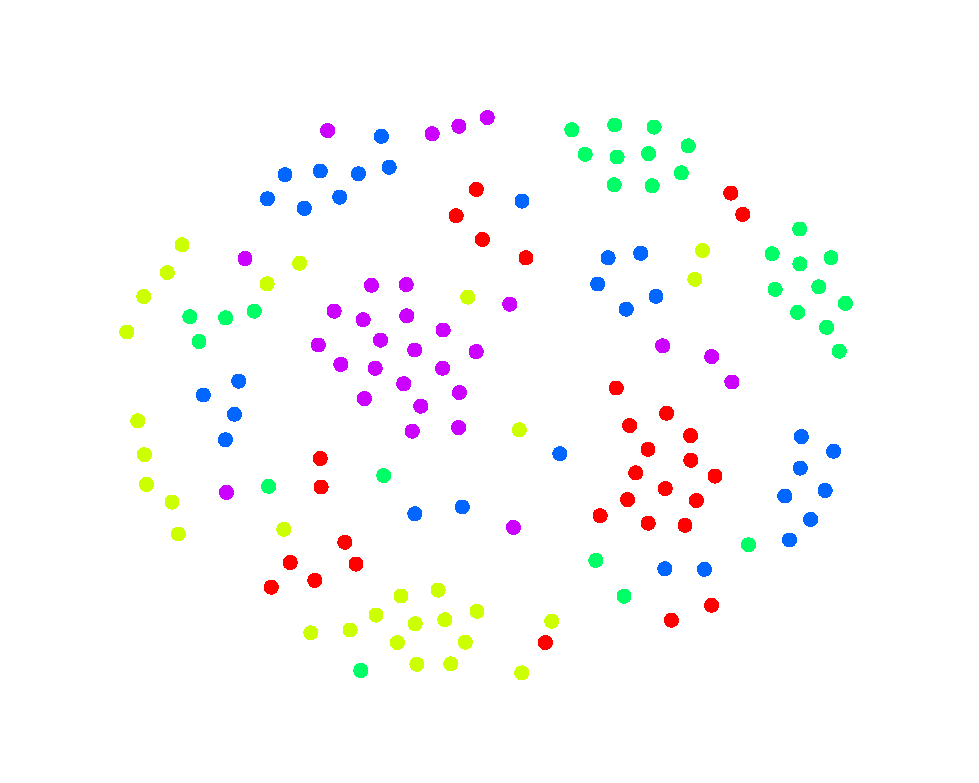
\includegraphics[width=0.15\paperwidth]{05types-3.pdf}}
  \fbox{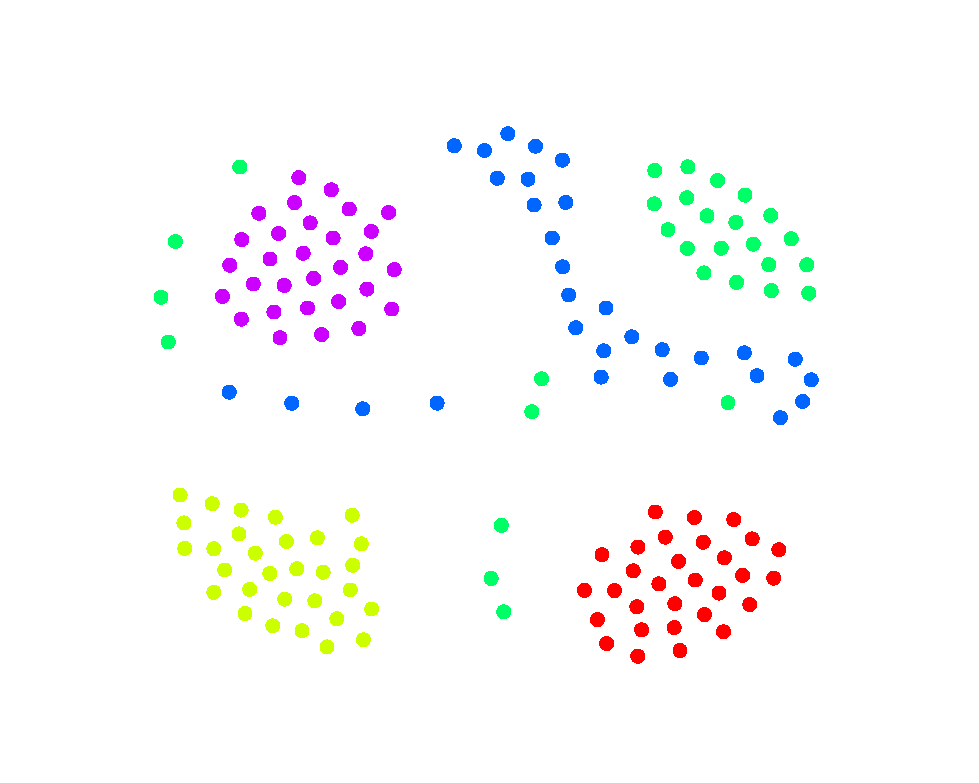
\includegraphics[width=0.15\paperwidth]{05types-4.pdf}}
  \fbox{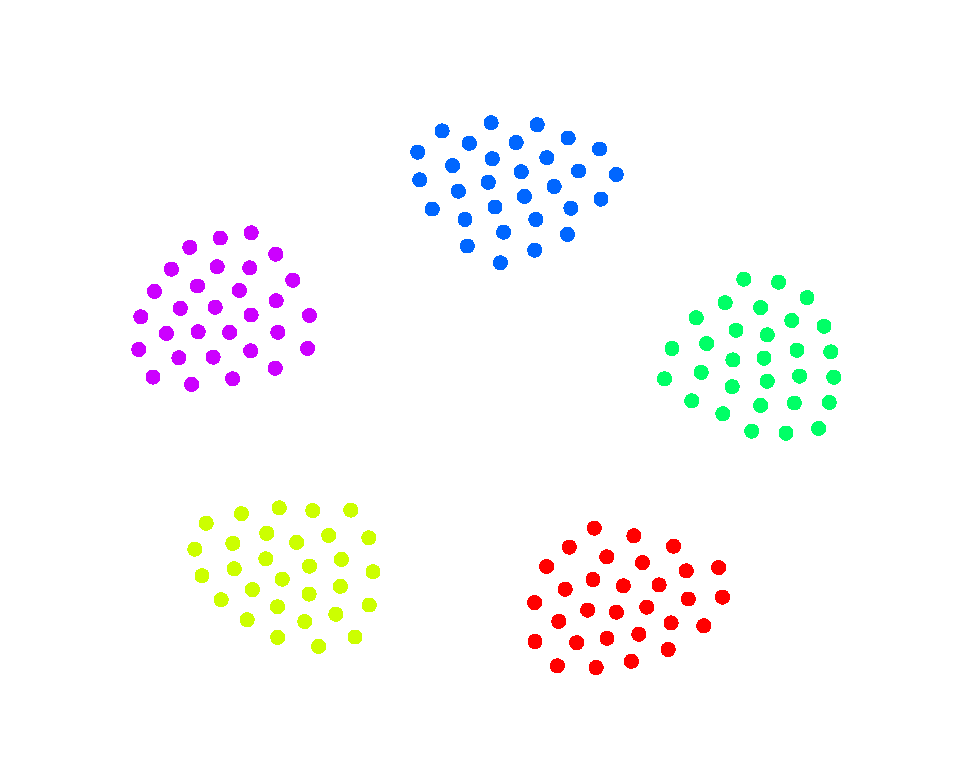
\includegraphics[width=0.15\paperwidth]{05types-5.pdf}}}
\subfigure[10 heterogeneous types.]{
  \fbox{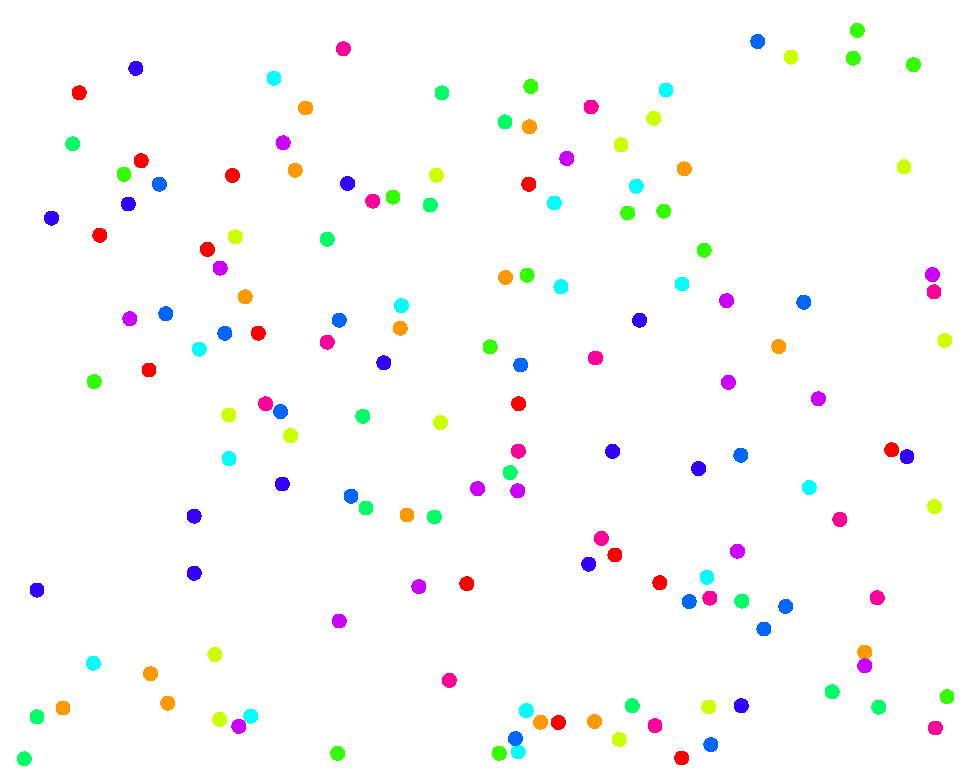
\includegraphics[width=0.15\paperwidth]{10types-1.pdf}}
  \fbox{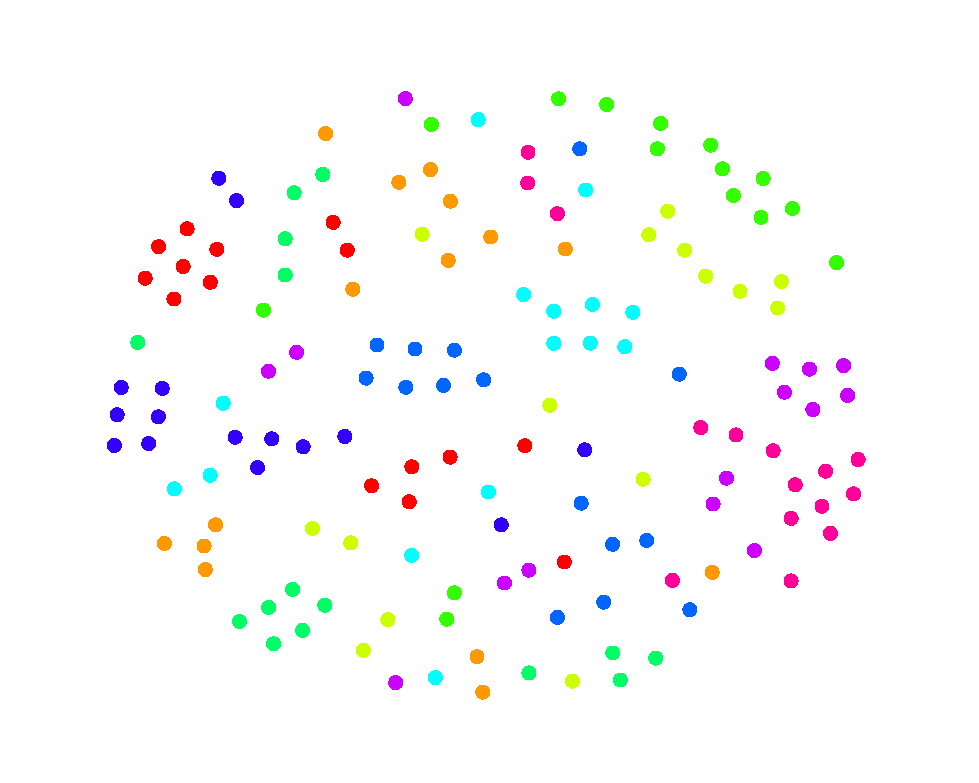
\includegraphics[width=0.15\paperwidth]{10types-2.pdf}}
  \fbox{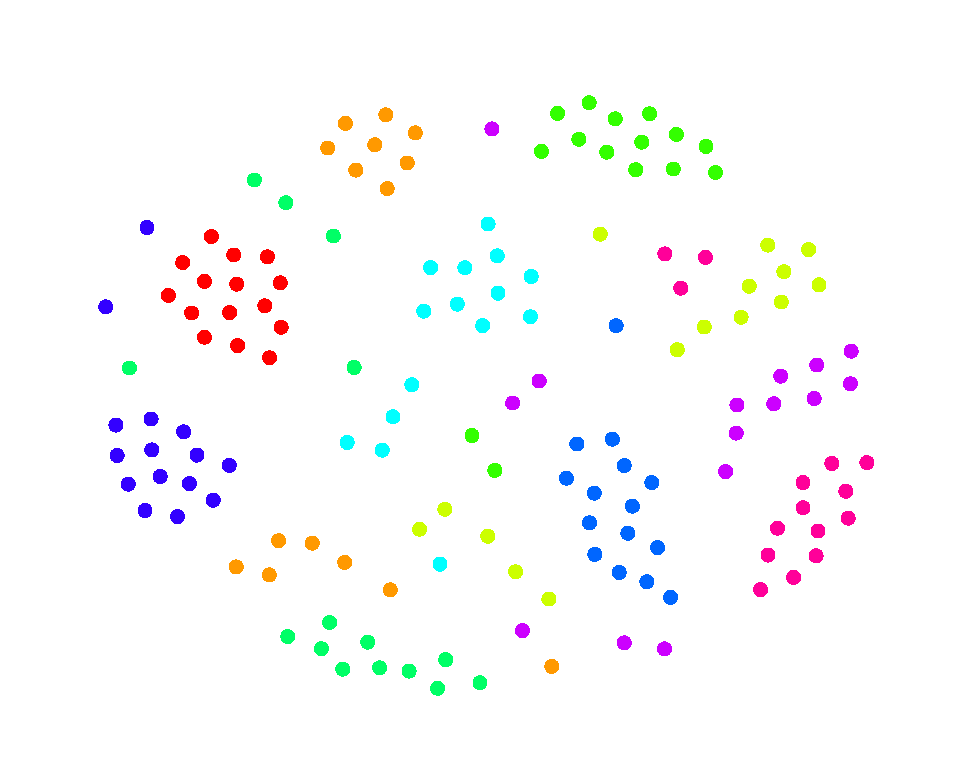
\includegraphics[width=0.15\paperwidth]{10types-3.pdf}}
  \fbox{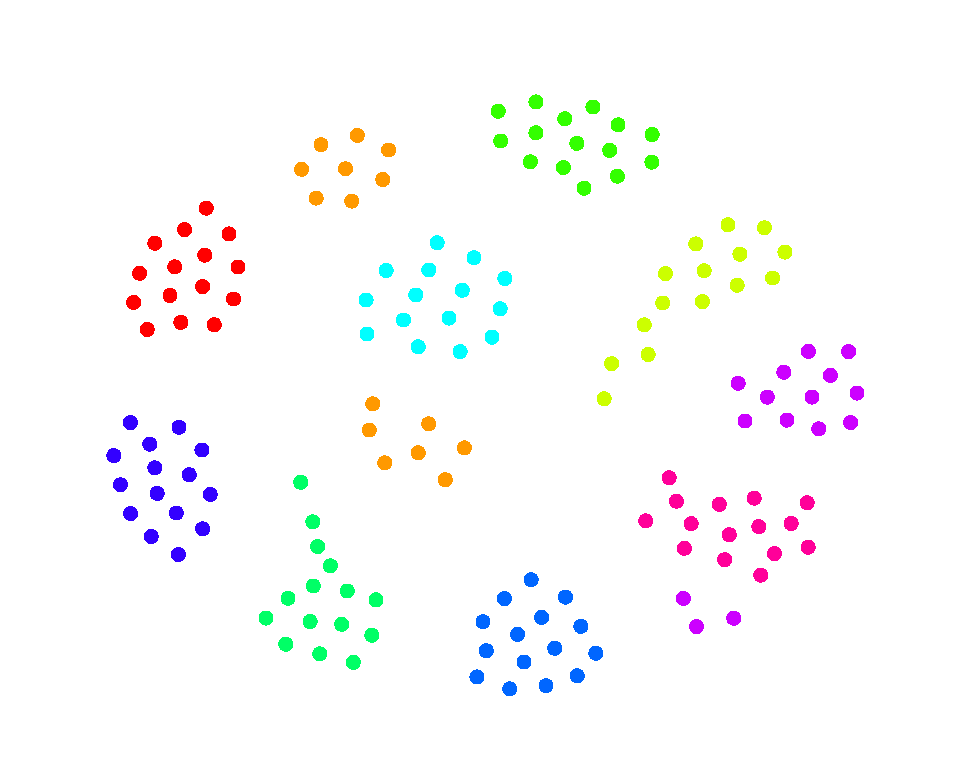
\includegraphics[width=0.15\paperwidth]{10types-4.pdf}}
  \fbox{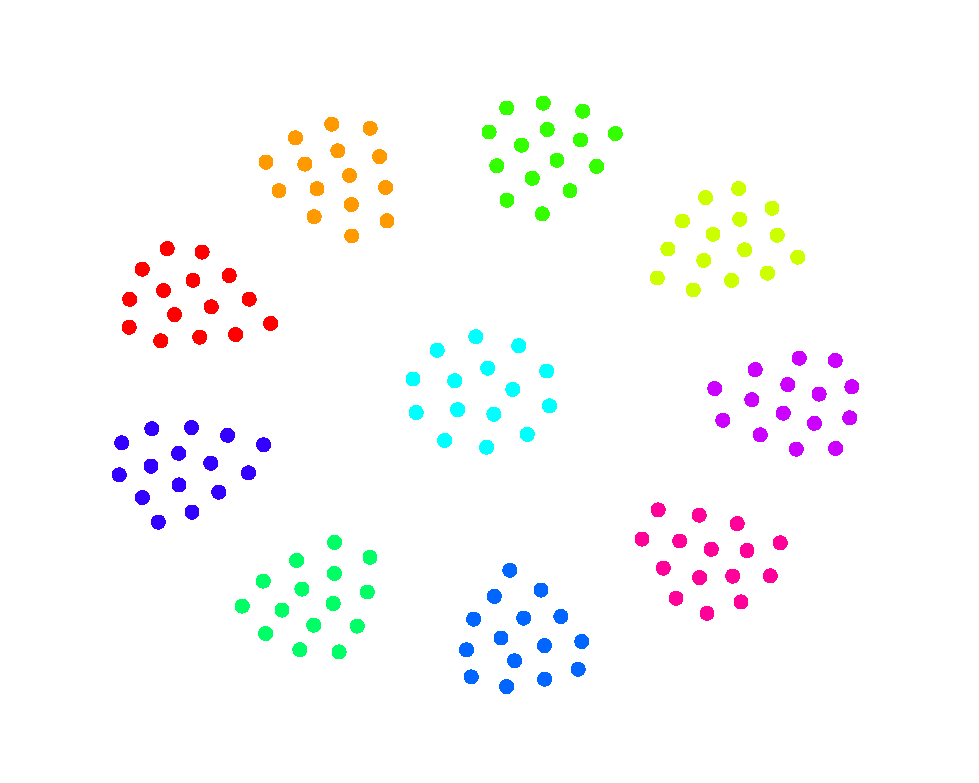
\includegraphics[width=0.15\paperwidth]{10types-5.pdf}}}
\subfigure[15 heterogeneous types.]{
 \fbox{ 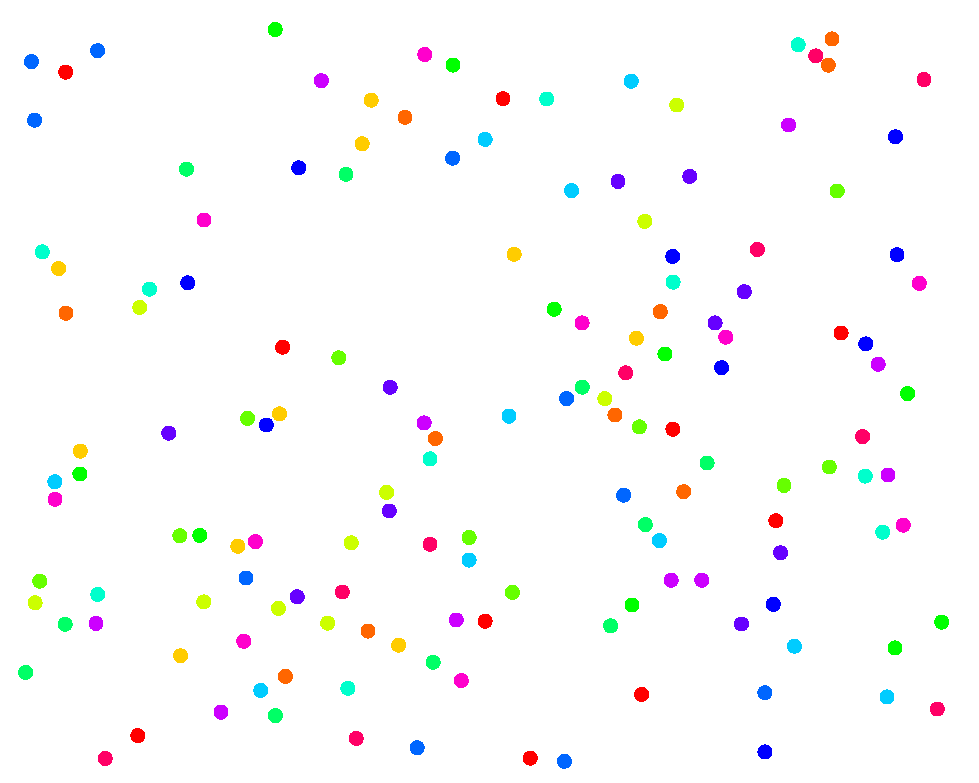
\includegraphics[width=0.15\paperwidth]{15types-1.pdf}}
  \fbox{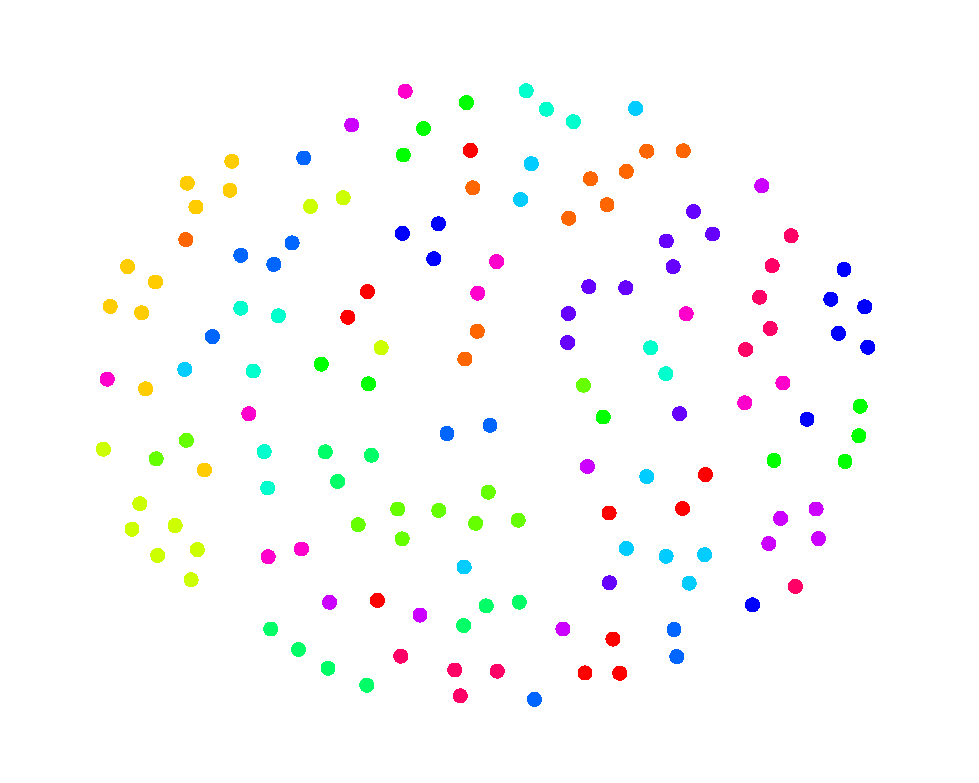
\includegraphics[width=0.15\paperwidth]{15types-2.pdf}}
  \fbox{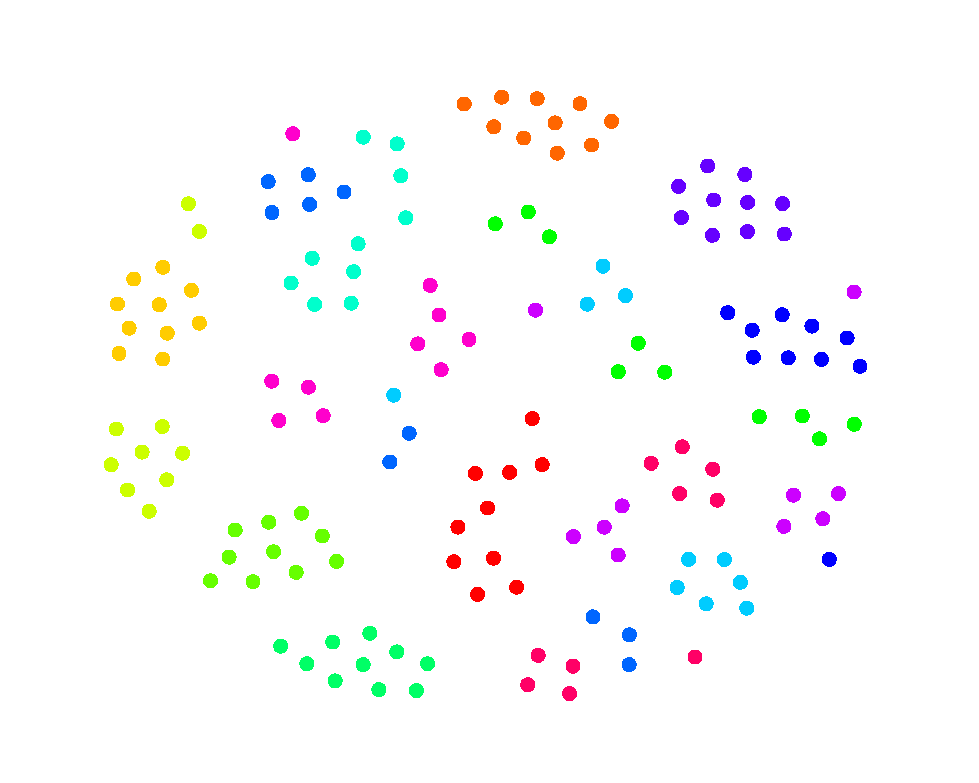
\includegraphics[width=0.15\paperwidth]{15types-3.pdf}}
  \fbox{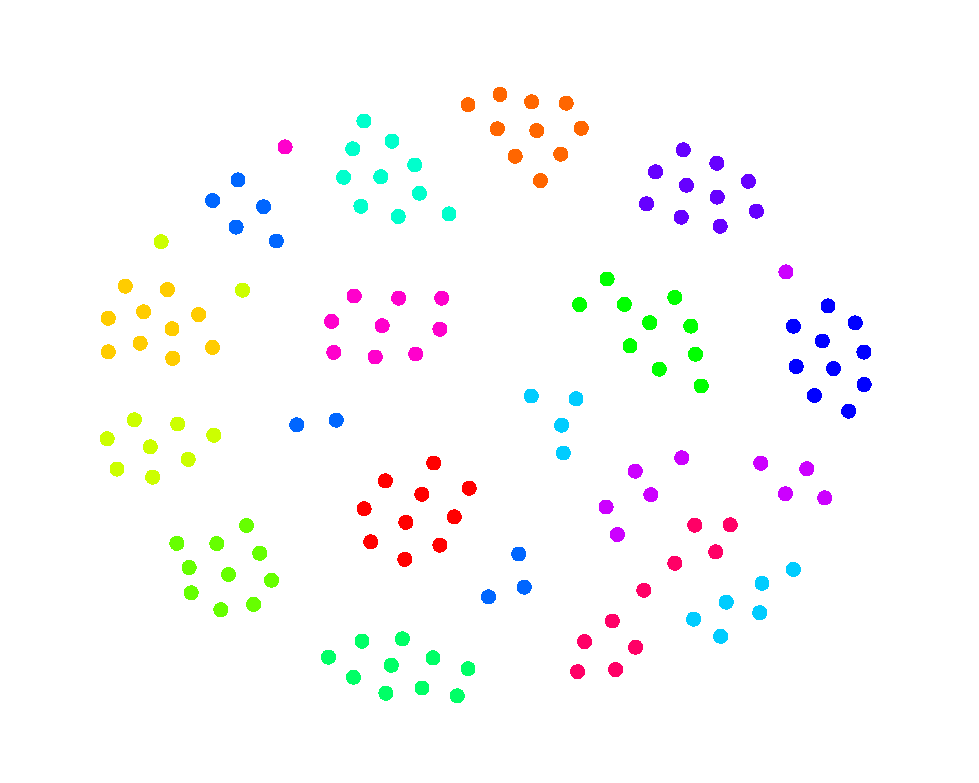
\includegraphics[width=0.15\paperwidth]{15types-4.pdf}}
  \fbox{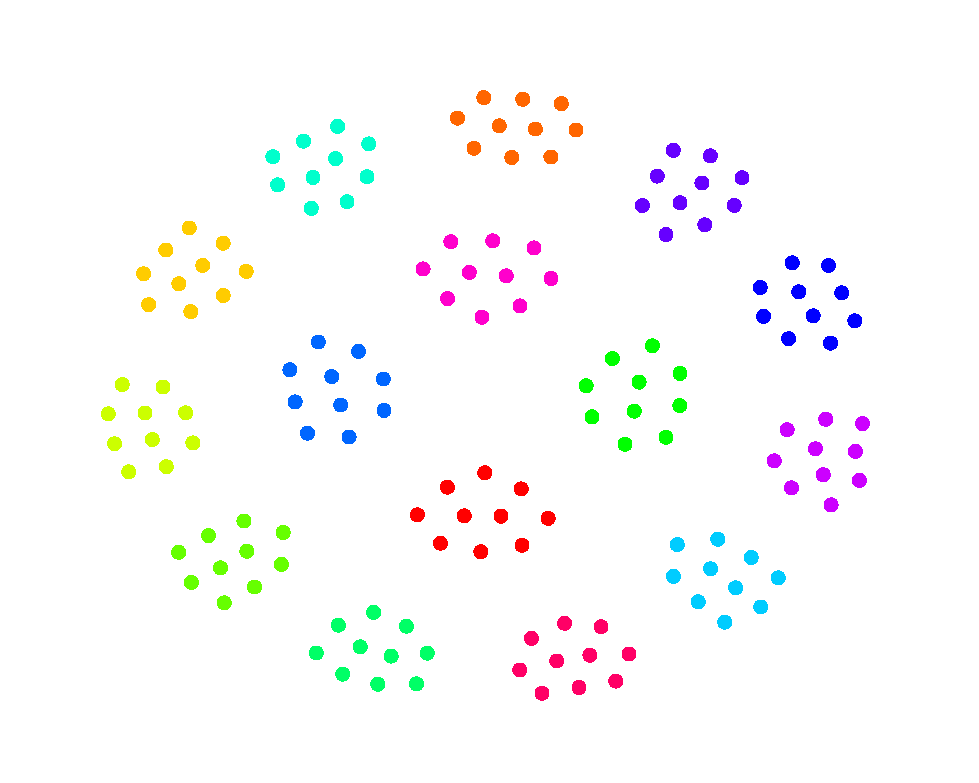
\includegraphics[width=0.15\paperwidth]{15types-5.pdf}}}
\caption{Snapshots of simulated executions with 150 robots and a
  varying number of heterogeneous types. In each sequence, the initial
  configuration is depicted on the left, whereas the final
  configuration is displayed on the right. Each robot type is
  represented by a different color.}
\label{fig:simulations}
\end{figure*}

We display in Figure \ref{fig:simulations} a series of snapshots from
particular instances of our experiments. Through a visual inspection,
we can see that similar robots quickly form clusters whose size grows
with time as other agents join them. Furthermore, interesting
geometrical patterns are organized at the stable state. We have also
observed two particular behaviors which might be difficult to notice
in the figures\footnote{An illustrative video of the simulations in
  Figures \ref{fig:simulations} and \ref{fig:3Dsimulations} can be
  found in the Multimedia Attachment of this paper.}: large ensembles
usually move to the outside of the main aggregate, the one that
embodies all agents of the system, and adjacent dissimilar clusters
form corridors which are used by agents of a third type to move at
higher speeds. Both of these behaviors are compelling because they
contribute to the opening of free spaces, whereby smaller clusters and
lone robots can take advantage of the situation and form larger
ensembles.

We have executed simulations in 3D space as well. Figure
\ref{fig:3Dsimulations} contains two images from the initial and final
configurations of experiments comprising 150 robots and a varying
number of agent types. Initial conditions were chosen exactly as in
the 2D simulations. The controller was able to achieve segregation,
and robots have displayed the same overall behavior as of their 2D
counterparts. Particularly, we have seen that it is easier for robots
to form clusters in this scenario because of the additional degree of
freedom, which allows agents to maneuver in new directions. Thus, in
the 3D case, it is unusual to find lone robots wandering towards their
cluster in later iterations, since larger clusters are aggregated more
quickly.

\subsection{Discussion}

Equation (\ref{eq:potential}) represents an important distinction
between our controller and Kumar's prior
work~\cite{Kumar:10}. Regarding their potential function, we noticed
that its gradient may vanish on the free space among adjacent
dissimilar clusters. This is the reason why our initial experiments,
which used their controller with multiple types, had often reached
undesirable local minima. Thus, by adding the quadratic term in
(\ref{eq:potential}), we have actually increased the norm of the
gradient and biased its direction, which allowed robots to keep moving
towards their respective cluster.

Desirable properties in swarm systems include scalability,
flexibility, and robustness~\cite{Sahin:04}. These are specially
important on applications in which robots may be inserted or removed
from the system dynamically. One of the main advantages of our
approach is that a robot does not need to know either how many agents
or how many types exist in the system. This is due to the second case
of (\ref{eq:dij}), in which we write $j \not \in \tau_k$ instead of $j
\in \Upsilon \setminus \tau_k$ as the former explicitly states that
robot $i$ needs to recognize only agents that are similar to
itself. Consequently, robots can be added or subtracted from the
system at any time.

\begin{figure}[thpb]
\centering
\subfigure[5 heterogeneous types.]{
  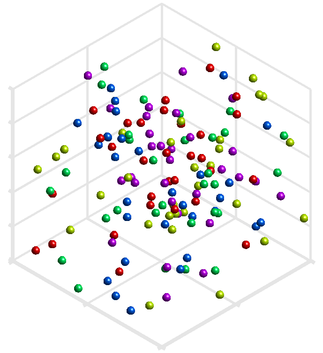
\includegraphics[width=0.33\columnwidth]{05types-3d1.png}\qquad
  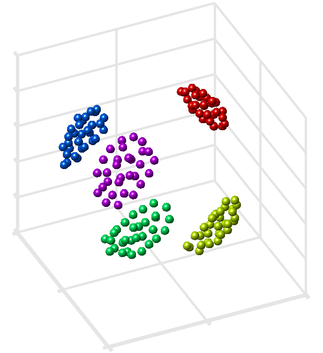
\includegraphics[width=0.33\columnwidth]{05types-3d2.png}}
\subfigure[10 heterogeneous types.]{
  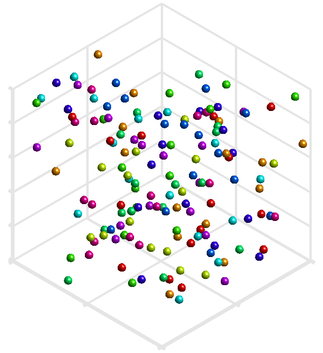
\includegraphics[width=0.33\columnwidth]{10types-3d1.png}\qquad
  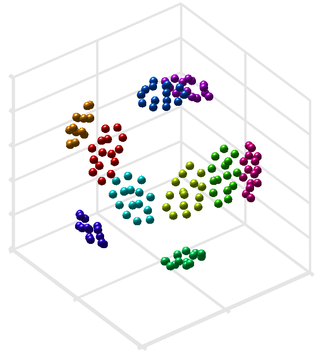
\includegraphics[width=0.33\columnwidth]{10types-3d2.png}}
\subfigure[15 heterogeneous types.]{
  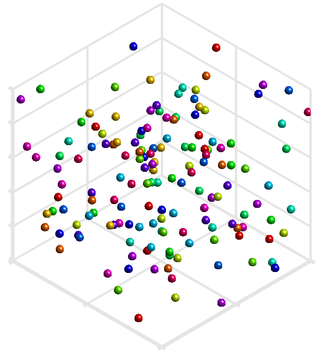
\includegraphics[width=0.33\columnwidth]{15types-3d1.png}\qquad
  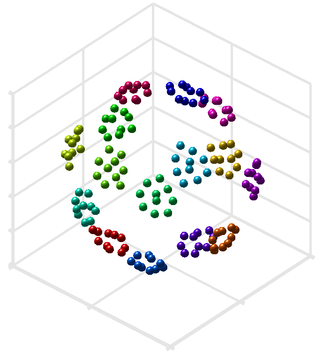
\includegraphics[width=0.33\columnwidth]{15types-3d2.png}}
\caption{Initial and final configurations of simulated experiments in
  3D space with 150 robots and a varying number of heterogeneous
  types. We apply an orthographic projection and slightly rotate the
  stable state to better depict the separation among clusters.}
\label{fig:3Dsimulations}
\end{figure}
\addtolength{\textheight}{-1.5cm}

As can be seen in (\ref{eq:controller}), our controller requires
global perception capabilities, i.e., each robot must know the
position and velocity of all agents. Thus, in spite of the robustness
of our approach, this constraint may hinder its applicability on
physical systems, as real sensors usually have constrained
capabilities which restrict robots to gather local information
only. This is also a limitation of the method
in~\cite{Kumar:10}. Regarding our metric, there is a possible drawback
in real robotic systems. In case of robot failures, the metric could
give unsatisfactory results for an otherwise well-segregated swarm,
since the location of a single agent can have a large impact on the
metric.

Although we have constrained our approach to balanced type partitions,
we executed some simulations with unbalanced partitions as well. In
these experiments, robots occasionally achieved segregation depending
on the relative balance of the partition, but several experiments
reached local minima when the type partition had been severely
unbalanced. In these local minima, robots were not segregated in the
sense of our proposed metric. This usually happens when robots cannot
reach their cluster as the attractive forces towards it are weaker
than those repelling them away from other agents. On the other hand,
these types of local minima in experiments with balanced type
partitions are not common. For example, among the $100$ experiments
with $15$ types presented in Figure \ref{fig:chull}, there was only
one instance which did not segregate. However, given the same initial
conditions, by choosing a larger value for $d_{AB}$ the controller was
able to achieve segregation. Thus, we think that this value should be
chosen according to how many robots and types exist in the system, as
larger numbers thereof may require wider corridors between dissimilar
clusters so that the gradient of the potential function will not
vanish.

Thus, we believe that, given a balanced type partition $\tau$, and
assuming that the underlying adjacency graph of the system is complete
at all times, for any initial condition that belongs to the level set
$\Omega_C$, there exists a finite value $r$ such that if
$\frac{d_{AB}}{d_{AA}} > r$ then $M(\mathbf{q}, \tau) \to 0$ as the
number of iterations approaches infinity. Nevertheless, it is still
necessary to gather more evidence in order to formally prove this
claim.

%We close this work with a proposition that is based on the evidences
%that we have gathered from our results. We present it as a conjecture
%since we have yet to prove its claim.
%\begin{conjecture}
%  Given a balanced type partition $\tau$, and assuming that the
%  underlying adjacency graph of the system is complete at all times,
%  for any initial condition that belongs to the level set $\Omega_C$,
%  there exists a finite value $r$ such that if $\frac{d_{AB}}{d_{AA}}
%  > r$ then $M(\mathbf{q}, \tau) \to 0$ as the number of iterations
%  approaches infinity.
%\end{conjecture}
%%%%%%%%%%%%%%%%%%%%%%%%%%%%%%%%%%%%%%%%%%%%%%%%%%%%%%%%%%%%%%%%%%%%%%%%%%%%%%%%
\section{CONCLUSION}
\label{sec:conclusion}

In this work, we proposed a controller that can sort a system of
multiple heterogeneous mobile robots into homogeneous clusters, such
that agents of similar types are segregated from dissimilar ones. We
based our approach on the differential potential concept, a
conceptualization of the mechanisms by which biological systems
achieve segregation. In this framework, agents experience distinct
magnitudes of potential when they interact with agents of different
types. We presented stability analyses and several experiments in 2D
and 3D scenarios, which demonstrated the effectiveness of the proposed
approach.

Despite the good results, we still see room for improvement. For
instance, our assumptions that robots have global sensing capabilities
may not hold in real scenarios, and severely unbalanced type
partitions may lead them to stable states that are not segregated in
the sense of our metric. Regarding the former, we think it would be
interesting to explore control laws and possibly other potential
functions that model local sensing into their methodologies, whereas
the latter could be tackled by employing non-symmetrical potential
functions. All in all, both problems can be regarded as a more general
one, and we believe that, by further studying these, our controller
can be improved to solve the segregation problem in a wider variety of
instances.

%\addtolength{\textheight}{-12cm} % This command serves to balance the column lengths
                                  % on the last page of the document manually. It shortens
                                  % the textheight of the last page by a suitable amount.
                                  % This command does not take effect until the next page
                                  % so it should come on the page before the last. Make
                                  % sure that you do not shorten the textheight too much.

%%%%%%%%%%%%%%%%%%%%%%%%%%%%%%%%%%%%%%%%%%%%%%%%%%%%%%%%%%%%%%%%%%%%%%%%%%%%%%%%



%%%%%%%%%%%%%%%%%%%%%%%%%%%%%%%%%%%%%%%%%%%%%%%%%%%%%%%%%%%%%%%%%%%%%%%%%%%%%%%%



%%%%%%%%%%%%%%%%%%%%%%%%%%%%%%%%%%%%%%%%%%%%%%%%%%%%%%%%%%%%%%%%%%%%%%%%%%%%%%%%
%\section*{APPENDIX}

%Appendixes should appear before the acknowledgment.

%\section*{ACKNOWLEDGMENT}

%%%%%%%%%%%%%%%%%%%%%%%%%%%%%%%%%%%%%%%%%%%%%%%%%%%%%%%%%%%%%%%%%%%%%%%%%%%%%%%%

\bibliographystyle{./IEEEtranBST/IEEEtran}
\bibliography{./IEEEtranBST/IEEEabrv,references}
\end{document}